\chapter{Background}
\label{ch.fundamentation}

	In the early days of electronic digital computing, John Von Neumann
	proposed an architectural model for computers to be easily programmable~\cite{von-neumann:model}.
	\autoref{fig:neumann} pictures the model scheme.
	The \cpu, also called core, loads instructions and data from an \mmu,
	dealing with inputs and generating outputs from/to I/O Devices.
	Modern processors still follow this model, but some components and
	behaviors are specialized or replicated to increase performance.

	\begin{figure}[!tb]
		\centering%
		\caption{Von Neumann Architecture Model.}%
		\label{fig:neumann}%
		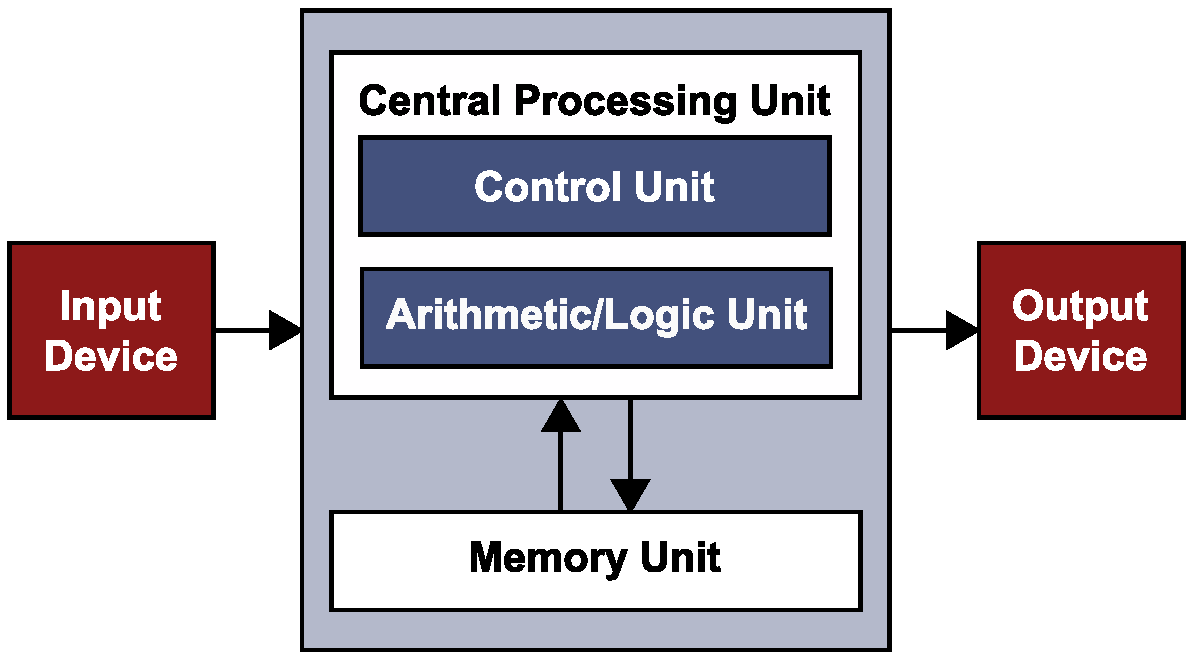
\includegraphics[width=.7\textwidth]{neumann.pdf}%
		\fonte{Adapted from \citeonline{tanenbaum:4ed}.}%
	\end{figure}
	
	According to \citeonline{tanenbaum:4ed}, there are three models of
	modern multiple processor architectures.
	A shared-memory multiprocessor, a message-passing multicomputer, and a wide
	area distributed system.
	In this chapter, we present the background of multiple processor systems from
	a hardware and software perspective.
	Specifically, \autoref{sec.multiprocessors} and \autoref{sec.multicomputers} addresses
	details about shared-memory multiprocessors and message-passing multicomputers, respectively.
	Subsequently, \autoref{sec.mppa} presents the \mppa processor.
	Finally, \autoref{sec.nanvix} shows an overview of Nanvix \os and the
	three levels of abstraction designed for \lightweight \manycores processors.

	\section{Multiprocessors}
	\label{sec.multiprocessors}

		A shared-memory multiprocessor is a computer system in which two or more \cpus
		share full access to a common \ram~\cite{tanenbaum:4ed}.
		The ability to run execution streams in parallel intensifies the concurrency
		issues that already existed in multi-tasking single-core processors.
		The competition of different cores for shared resources may result in
		inconsistent outputs or even in an inconsistent \os state.
		For instance, when a thread writes a value to a global variable and
		reads a different value.
		Moreover, some architectures integrate heterogeneous cores introducing
		portability and programmability problems too.
		So, low-level software, such as \os kernels and runtimes, needs to handle
		those issues and provide management systems to user-level.

		\subsection{Multiprocessor Hardware}
		\label{sec.multiprocessor-hw}

			The multiprocessors can be usually classified using memory access
			and workflow properties.
			In the first place, the access time to different memory addresses
			split multiprocessors into two groups.
			On the one hand, the group of systems that can read a memory word
			as fast as every other memory word are called \uma multiprocessors.
			On the other hand, \numa multiprocessors do not have this property.

			The firsts \uma multiprocessors were bus-based architectures where
			the \cpu wait for the bus channel stays free to perform a memory
			access, as illustrated in \autoref{fig:uma_a}.
			When the number of cores scale, the bus traffic becomes a
			bottleneck of the system.
			To solve this problem, a small but fast memory level, called cache,
			is added to each \cpu, as depicted in \autoref{fig:uma_b}.
			The cache allowed successive readings to be resolved locally,
			reducing traffic to the main memory.
			However, many problems of inconsistency and ordering of operations
			on memory arose with the advent of caches.
			For instance, when a write operation dirties a memory address in
			a particular cache, this change must be notified to all other caches.
			Equally important, it is necessary to ensure a specific order in
			the concurrent operations on a given address through different caches.
			The protocols that guarantee these properties are called cache-coherence
			protocols~\cite{tanenbaum:4ed}.

			\begin{figure}[!tb]
				\centering%
				\caption{Two Bus-Based \uma Multiprocessor Examples.}%
				\label{fig:uma}%

				\subcaptionminipage[fig:uma_a]%
					{.4\linewidth}%
					{Without caching.}%
					{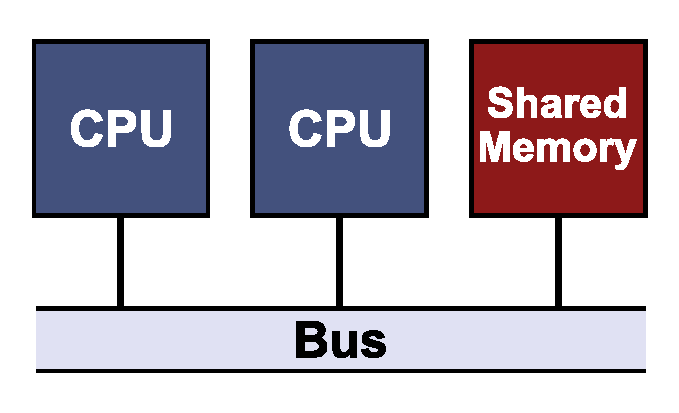
\includegraphics[width=\linewidth]{uma_a.pdf}}%
				\hspace{1.5cm}%
				\subcaptionminipage[fig:uma_b]%
					{.4\linewidth}%
					{With caching.}%
					{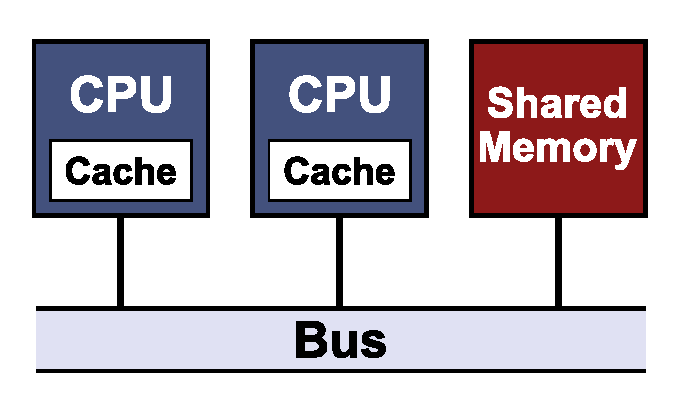
\includegraphics[width=\linewidth]{uma_b.pdf}}%

				\fonte{Adapted from \citeonline{tanenbaum:4ed}.}%
			\end{figure}

			Nevertheless, the number of cores in \uma multiprocessors are limited
			to a few dozens of \cpus.
			Thus, to allow hundreds of cores to communicate, \autoref{fig:numa} illustrates
			as that \numa machines provide a single address space visible to all \cpus
			through an interconnection network.
			Therefore, distributing a virtual memory space among local physics memories,
			the access is guaranteed via load and store instructions.
			Although the time to access the remote memory is slower than to local ones,
			this granted that all \uma programs will be able to run on \numa machines
			but with worse performance.

			\begin{figure}[!tb]
				\centering%
				\caption{\numa Multiprocessor Example.}%
				\label{fig:numa}%
				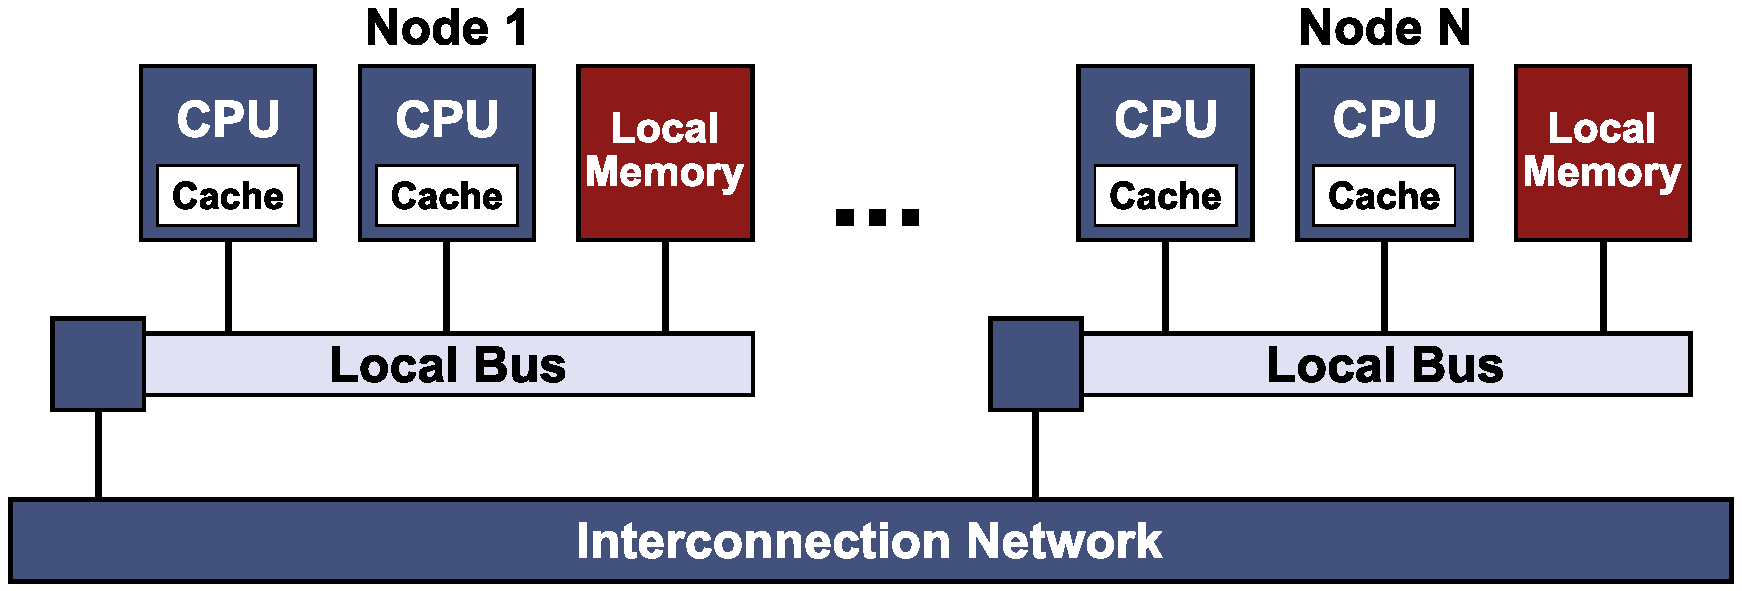
\includegraphics[width=.7\textwidth]{numa.pdf}%
				\fonte{Adapted from \citeonline{tanenbaum:4ed}.}%
			\end{figure}

			In the second place, the workflow classification proposed by \citeonline{flynn:1972},
			split multiprocessors architecture based on the number of concurrent
			instruction and data streams available, as depicted in \autoref{fig:flynn}.
			First, the most straightforward class, \sisd describes a sequential
			machine which exploits no parallelism in either the instruction or
			data streams, like older uniprocessor machines.
			Second, \simd uses multiple functional units to replicate and operate
			a single instruction over multiples different data streams, like \gpu.
			Third, the most uncommon class, \misd describe multiprocessors that
			apply multiple instructions streams over one data stream.
			Systems that need fault tolerance uses theses multiprocessors, like
			modern flight control systems.
			Finally, a \mimd architecture has multiple processors simultaneously
			executing different instruction on different data, like \xeonphi.

			\begin{figure}[!tb]
				\centering%
				\caption{Flynn's taxonomy.}%
				\label{fig:flynn}%

				\subcaptionminipage[fig:flynn-sisd]%
					{.4\linewidth}%
					{Single Instruction Single Data.}%
					{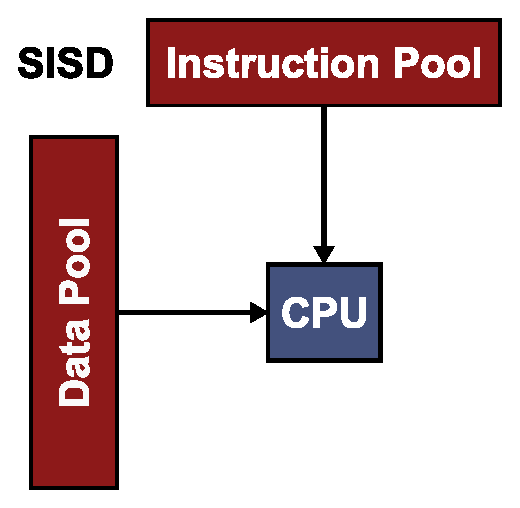
\includegraphics[width=.8\linewidth]{sisd.pdf}}%
				\hspace{1cm}%
				\subcaptionminipage[fig:flynn-simd]%
					{.4\linewidth}%
					{Single Instruction Multiple Data.}%
					{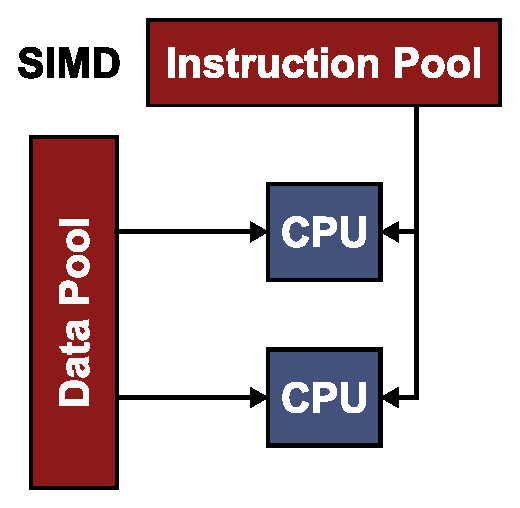
\includegraphics[width=.8\linewidth]{simd.pdf}}%

				\subcaptionminipage[fig:flynn-misd]%
					{.4\linewidth}%
					{Multiple Instruction Single Data.}%
					{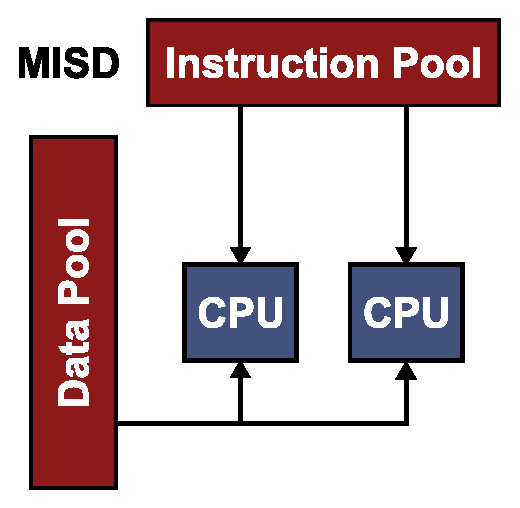
\includegraphics[width=.8\linewidth]{misd.pdf}}%
				\hspace{1cm}%
				\subcaptionminipage[fig:flynn-mimd]%
					{.4\linewidth}%
					{Multiple Instruction Multiple Data.}%
					{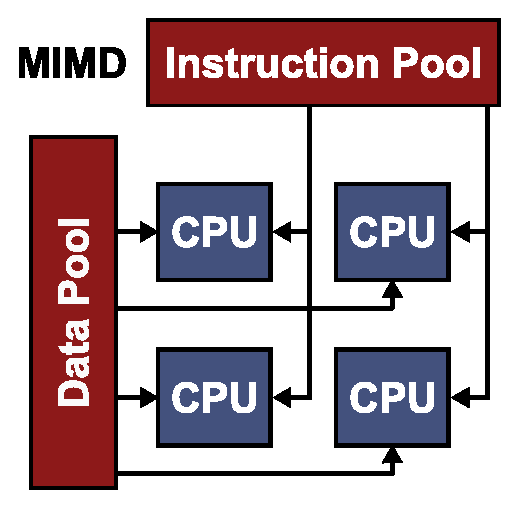
\includegraphics[width=.8\linewidth]{mimd.pdf}}%

				\fonte{Adapted from \citeonline{url:flynn}.}%
			\end{figure}

			Currently, two categories of multiprocessors attract attention, the \cmp and \mpsoc.
			\cmps are multicore commercials, which follow a symmetric architecture,
			integrating two or more identical cores into a single die.
			They can have private or shared cache levels, and always share access
			to the \ram.
			Alternatively, \mpsocs are designed with an asymmetric architecture,
			have in addition to the main cores, specialized \cpus in particular
			functions, \eg audio and video encoders, encryption, becoming truly
			complete computer systems on a single chip.
			All these cores are linked to each other by an on-chip network-based
			communications subsystem, called \noc.
			The \noc improves scalability and power consumption compared to other
			communication subsystem designs.

		\subsection{Multiprocessor Operating Systems}
		\label{sec.multiprocessor-os}

			\oss are a fundamental part of any computer system.
			They act as an intermediary between users and hardware, with the
			purpose to provide an environment in which users can run programs
			in a conveniently and efficiently manner~\cite{Silberschatz:9ed}.
			Many \os approaches exist in multiprocessor systems.
			In particular, three of them express accurately the difficulties
			of developing \oss targeting the concurrency issues existing in
			such systems.
			Those models are called Replicated, Master-Slave, and Symmetric \os.

			The Replicated Model is the simplest way to develop an \os for a
			parallel architecture.
			It only needs to replicate all the internal \os structures for each core.
			\autoref{fig:replicated-os} illustrates how this model allocates fixed memory spaces
			between the cores, giving each of them its private \os.
			The system calls are performed by the calling \cpu, avoiding concurrency issues.
			Also, a producer-consumer model is sufficient for two different \cpus to communicate.

			\begin{figure}[!tb]
				\centering%
				\caption{Replicated \os Model.}%
				\label{fig:replicated-os}%
				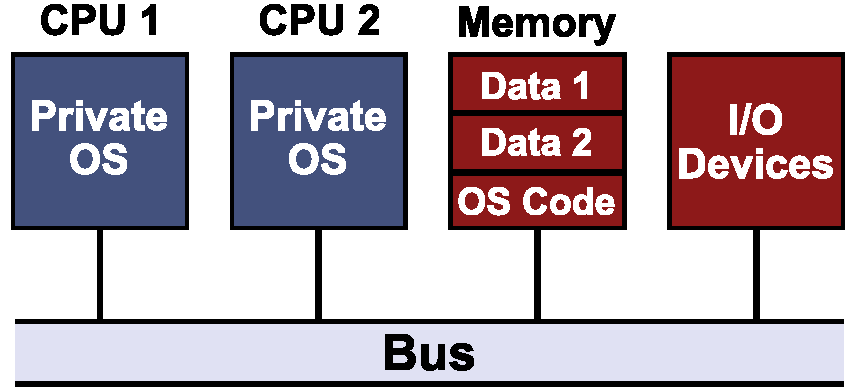
\includegraphics[width=.55\textwidth]{replicated-os.pdf}%
				\fonte{Adapted from \citeonline{tanenbaum:4ed}.}%
			\end{figure}

			However, this model has imperceptible aspects~\cite{tanenbaum:4ed}.
			First, since each \cpu has its own process and page tables, it is impossible
			to optimize the use of resources.
			For instance, if many of processes are waiting for use an overloaded \cpu,
			it is impossible to migrate them to an available \cpu.
			Second, operations with I/O devices can introduce inconsistency problems
			such as the same disk block operated by different \cpus.
			Finally, replication of the internal \os structures makes this model
			impractical for systems with memory constraints.

			The Master-Slave model began to attract attention with the return of
			processors with no cache coherence.
			As \autoref{fig:master-slave-os} pictures, there is only one copy of
			the internal \os structures, and they all belong to a single \cpu, called master.
			In this way, all system calls performed by a worker \cpu, called slave,
			are redirected to the master.
			With these changes, this model solves the problems of the previous model
			by using only one copy of the data structures.
			For illustration, processes and memory pages can be scheduled and
			distributed dynamically to any \cpus.
			However, when adopting a centralized approach, the master can become
			the bottleneck of the system if it can not handle the number of the
			incoming requisitions.

			\begin{figure}[!tb]
				\centering%
				\caption{Master-Slave \os Model.}%
				\label{fig:master-slave-os}%
				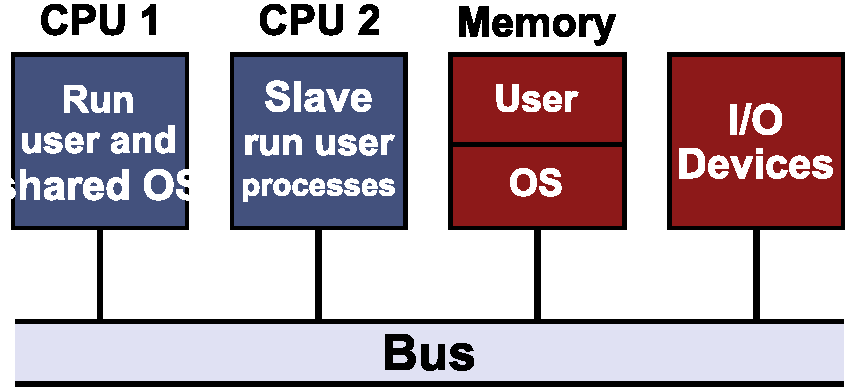
\includegraphics[width=.55\textwidth]{master-slave-os.pdf}%
				\fonte{Adapted from \citeonline{tanenbaum:4ed}.}%
			\end{figure}

			Finally, the Symmetric model, called \smp, eliminates the centralization
			problem of the foregoing model, as illustrated in \autoref{fig:smp-os}.
			So, there is still only one copy of the \os structures but shared in memory.
			When a \cpu makes a system call, it loads the structures and operates on them.
			Consequently, processes and memory pages also continue to be dynamically balanced.
			The difficulties introduced by this model lie in concurrency for \os structures.
			Depending on how the critical regions are managed, the performance of the system
			may be equivalent to the Master-Slave model. So the hardest part is breaking the
			\os into critical regions that will run on different \cpus, where one core does
			not affect the execution of another or fall into a deadlock~\cite{tanenbaum:4ed}.
			Besides, if the hardware does not support cache coherence, the process of
			invalidating the cache may also introduce serious performance problems in \oss of this type.

			\begin{figure}[!tb]
				\centering%
				\caption{Symmetric \os Model.}%
				\label{fig:smp-os}%
				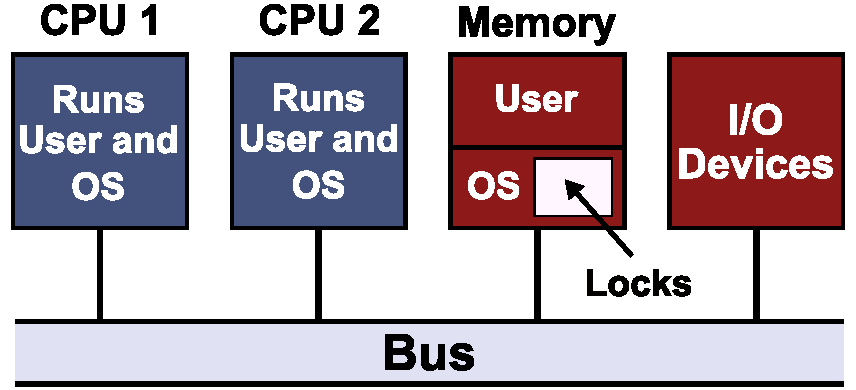
\includegraphics[width=.55\textwidth]{symmetric-os.pdf}%
				\fonte{Adapted from \citeonline{tanenbaum:4ed}.}%
			\end{figure}

			As it can be noted, the software is always lagging behind the constant hardware advances.
			Many solutions may work very well in specific contexts but should be chosen with care.
			In some cases, in order to extract the maximum performance from a system, it will be
			necessary to redesign the whole software stack from scratch.

	\section{Multicomputers}
	\label{sec.multicomputers}

		Increasing the number of cores and still providing a shared memory in a
		single die is very expensive and challenging.
		However, it is more simple and cheap to interconnect more straightforward
		computers in a high-speed network. The result is a clustered architecture.
		Despite the problem of developing networks and high-speed interfaces
		for communication of the nodes, it is analogous to the problem of
		providing a shared memory in multiprocessors.
		Nevertheless, the expected communication times will be in the
		microseconds, as opposed to nanoseconds of the multiprocessors,
		making things simpler~\cite{tanenbaum:4ed}.

		\subsection{Multicomputer Hardware}
		\label{sec.multicomputers-hw}

			A multicomputer node can be considered as an elementary computer, with one or
			more multiprocessors, local \ram and I/O devices.
			In many cases, there is no need for monitors or keyboards, only the
			network interface.
			In this way, it is possible to integrate hundreds or even thousands
			of nodes providing the vision of a single computer.

			A switch set is organized into different topologies to interconnect
			the nodes of a multicomputer.
			As illustrated in \autoref{fig:net-topologies}, there are a
			variety of topologies with their own characteristics.
			For instance, commercial multicomputer usually uses bi-dimensional
			topologies such as \textit{grid} or \textit{mesh} because they present
			regular behavior and can scale easily.
			When the goal is to provide higher fault tolerance, in addition to the
			smaller path between two points, the \textit{torus} variant implement
			connections between the extreme points of the \textit{grid}.
			Even multi-dimensional topologies can be used, all depending on the
			characteristics expected from the network.

			\begin{figure}[!tb]
				\centering%
				\caption{Network Topologies Examples.}%
				\label{fig:net-topologies}%

				\subcaptionminipage[fig:net-start]%
					{.25\linewidth}%
					{Star.}%
					{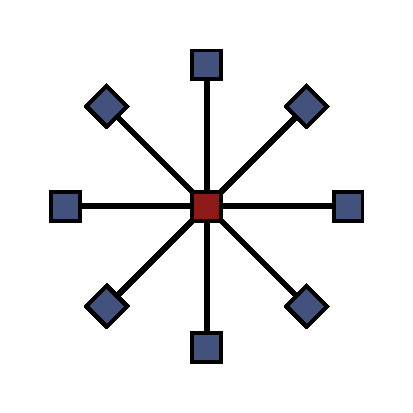
\includegraphics[width=\linewidth]{net-star.pdf}}%
				\hspace{1cm}%
				\subcaptionminipage[fig:net-ring]%
					{.25\linewidth}%
					{Ring.}%
					{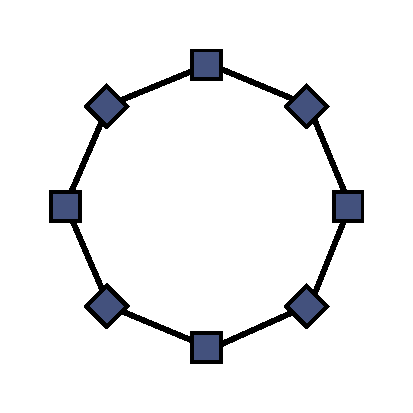
\includegraphics[width=\linewidth]{net-ring.pdf}}%
				\hspace{1cm}%
				\subcaptionminipage[fig:net-grid]%
					{.25\linewidth}%
					{Grid.}%
					{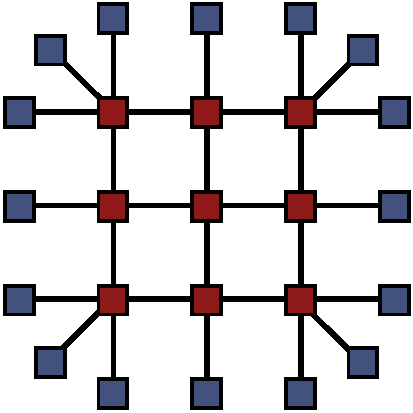
\includegraphics[width=\linewidth]{net-grid.pdf}}%

				\subcaptionminipage[fig:net-torus]%
					{.25\linewidth}%
					{Torus.}%
					{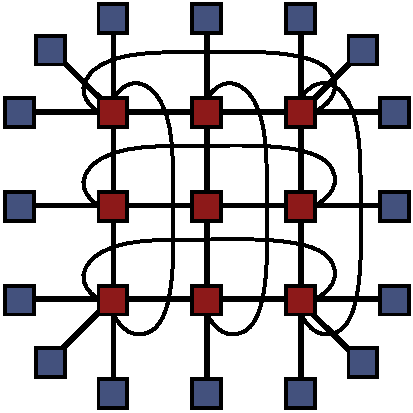
\includegraphics[width=\linewidth]{net-torus.pdf}}%
				\hspace{1cm}%
				\subcaptionminipage[fig:net.grid-3d]%
					{.25\linewidth}%
					{Grid 3D.}%
					{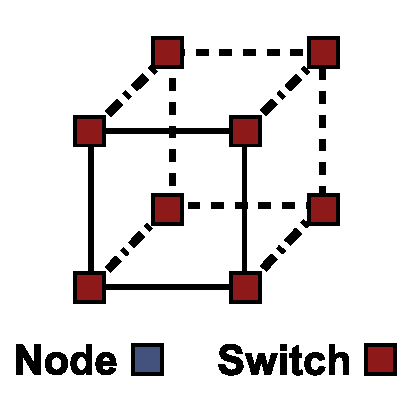
\includegraphics[width=\linewidth]{net-3d.pdf}}%

				\fonte{Adapted from \citeonline{tanenbaum:4ed}.}%
			\end{figure}

			There are two types of switching schemes in the multicomputer network.
			The \textit{store-and-forward packet} switching scheme breaks the message
			into fixed-size packets.
			The packets are copied and moved between the switches following a
			routing algorithm until they reach the destination.
			Although flexible and efficient, this scenario can generate a variable
			latency in packet delivery.
			The other scheme, called \textit{circuit switching}, performs a resource
			allocation protocol through all path from source to the destination.
			This protocol ensures a steady communication stream, although the
			slow start and possible sub-utilization of the resources.

		\subsection{Low-Level Communication Software}
		\label{sec.multicomputers-low-sw}

			Multicomputer nodes are interconnected to each other through network interfaces.
			Because these boards are built and connected to \cpus and \ram,
			they have substantial impacts on system performance and \os design.
			Virtually, interfaces have enough \ram space to receive/send packets.
			If this address space is actually in main memory, we fall into the same
			problem of multiprocessors in the struggle for the use of the bus channel.
			Thus, in general, network cards have a dedicated memory so as not to
			generate bottlenecks in access to main memory, as illustrated in \autoref{fig:multicomputer}.

			\begin{figure}[!tb]
				\centering%
				\caption{Simple Multicomputer Example.}%
				\label{fig:multicomputer}%
				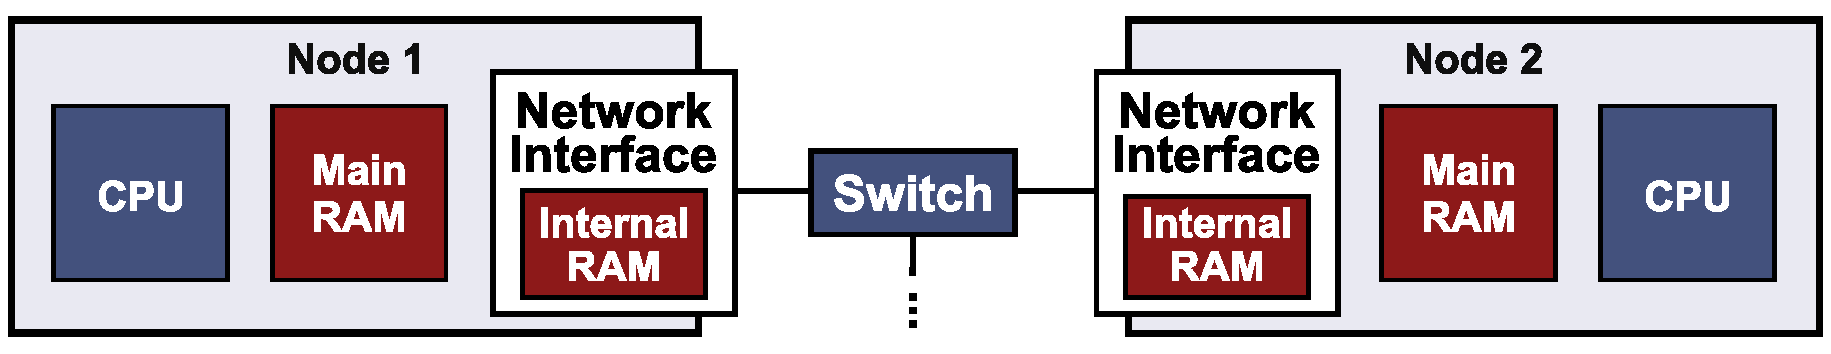
\includegraphics[width=.8\textwidth]{multicomputer.pdf}%
				\fonte{Adapted from \citeonline{tanenbaum:4ed}.}%
			\end{figure}

			However, excessive packet copying can degrade the performance of the system.
			In an ideal scenario, four end-to-end copies would be needed:
			(i) from the \ram of the sender to the interface memory;
			(ii) from the interface to the network;
			(iii) from the network to the memory of the target interface, and, finally,
			(iv) to the \ram of the recipient.
			Notwithstanding, the number of copies may increase further, depending on
			how the \os implements communication services on available hardware.
			For instance, mapping the interface into the kernel address space
			rather than the user-space, an extra copy to an internal kernel
			buffer is required.
			Thus, for performance reasons, modern systems already map the interfaces
			to user-space address even as new concurrency issues arise over
			communication resources.

			Processors may also have one or more \cpus specialized in
			communication procedures, called \dma.
			\dmas can make copies between system memories, send/receive packets
			without the main \cpus intervention.
			This reduces considerably wasted cycles due to network interfaces
			communication and/or main memory access bottlenecks.
			However, such intermediate copies lead to overhead on system structures,
			such as cache, \tlb, or page management.
			Furthermore, this introduces concurrency issues in the interaction between
			\cpus and existing \dma channels.

		\subsection{User-Level Communication Software}
		\label{sec.multicomputers-user-sw}

			The low-level mechanisms discussed above allow cores on different
			computers to communicate through the messages exchange by
			send/receive primitives.
			However, it is still the responsibility of the user to define the
			required parameters to perform such operations.
			In order for the user to send a message, he must inform the
			localization of the message, its size, and the identifier of the
			receiving interface.
			On the receiver side, the user must configure the interface with
			the location of sufficient memory space to receive the incoming message.

			\begin{figure}[!tb]
				\centering%
				\caption{Synchronous and Asynchronous Calls.}%
				\label{fig:calls-types}%

				\subcaptionminipage[fig:call-sync]%
					{.9\linewidth}%
					{Synchronous Call on Sender Node.}%
					{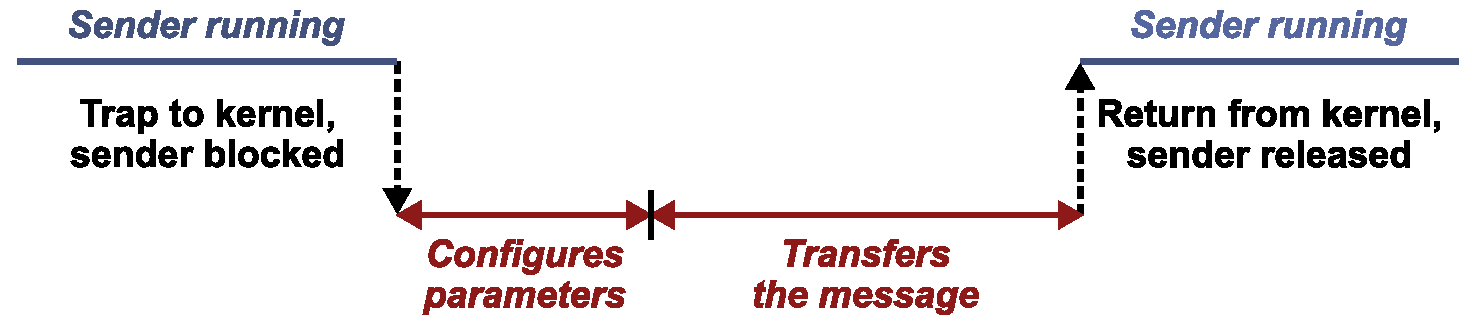
\includegraphics[width=\linewidth]{call-sync.pdf}}%

				\hfill

				\subcaptionminipage[fig:call-async]%
					{.9\linewidth}%
					{Asynchronous Call on Sender Node.}%
					{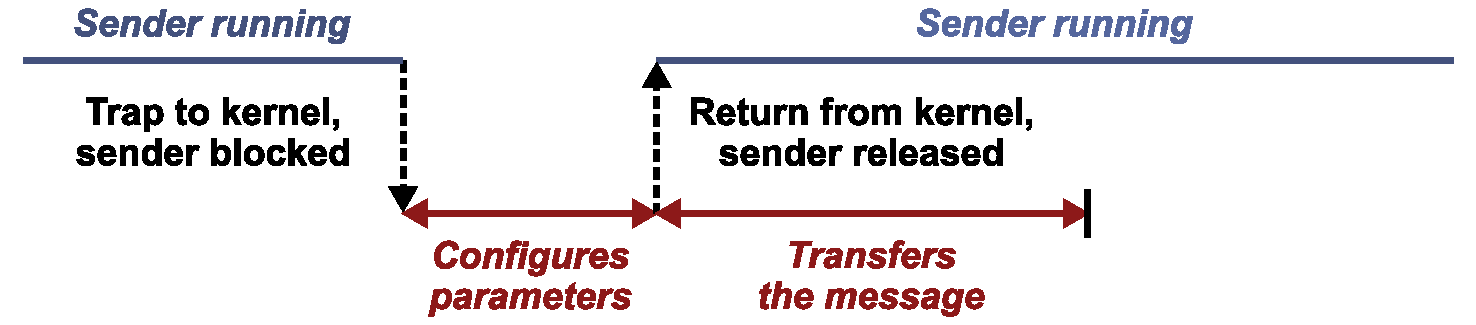
\includegraphics[width=\linewidth]{call-async.pdf}}%

				\fonte{Adapted from \citeonline{tanenbaum:4ed}.}%
			\end{figure}

			\autoref{fig:calls-types} illustrates the two approaches to implement
			these primitives, either through blocking or non-blocking calls.
			Blocking calls, called \textit{synchronous calls}, block the requesting \cpu
			until complete the procedure.
			Non-blocking calls, called \textit{asynchronous calls}, return control to the
			\cpu while the procedure is still in progress.
			Although asynchronous calls provide better performance than
			synchronous ones, they introduce some disadvantages where the sender/receiver
			cannot use the message buffer before the operation is complete.
			According to Tanenbaum~\cite{tanenbaum:4ed}, there are four ways to implement
			a send primitive:
			\begin{itemize}
				\item \textit{Blocking sending:} \cpu hibernates or schedules another
					process, while the message is transmitted;
				\item \textit{Non-blocking sending with copying:} realizes an extra copy of
					the message to a kernel buffer, degrading performance;
				\item \textit{Non-blocking sending with interrupt:} notifies the \cpu
					when the send finishes, where the buffer must remain untouchable,
					difficulting the programmability;
				\item \textit{\cow:} management of buffers to make an extra copy only
					when needed, but can copy unnecessarily.
			\end{itemize}

			Analogously, there are other four forms to implement a receive primitive:
			\begin{itemize}
				\item \textit{Blocking receive:} \cpu hibernates or schedules another
					process until a message is received;
				\item \textit{Non-Blocking receive with messages pool:} \cpu creates
					a buffer to store incoming messages, then consumes from it when
					there is some message available, requiring synchronization;
				\item \textit{Non-Blocking receive with Pop-up Threads:} creates a specific
					thread upon receiving a message to perform the necessary operations,
					but consumes resource for creating and destroying the thread;
				\item \textit{Non-Blocking receive with interrupt handlers:} the receiver
					is interrupted to execute a handler when receiving a message, resulting
					in a better performance than creating a thread but difficults
					the programmability.
			\end{itemize}

			Some of the implementation approaches may be hardware dependent.
			However, choosing the ideal approach is still the responsibility of the \os designer.
			Even so, the distributed nature of multicomputers forces a message-passing
			strategy regardless of what the hardware has to offer.

\section{MPPA-256 Lightweight Manycore Processor}
\label{sec.mppa}

	\begin{figure}[!tb]
		\centering%
		\caption{Architectural overview of the \mppa processor.}%
		\label{fig:mppa-arch}%
		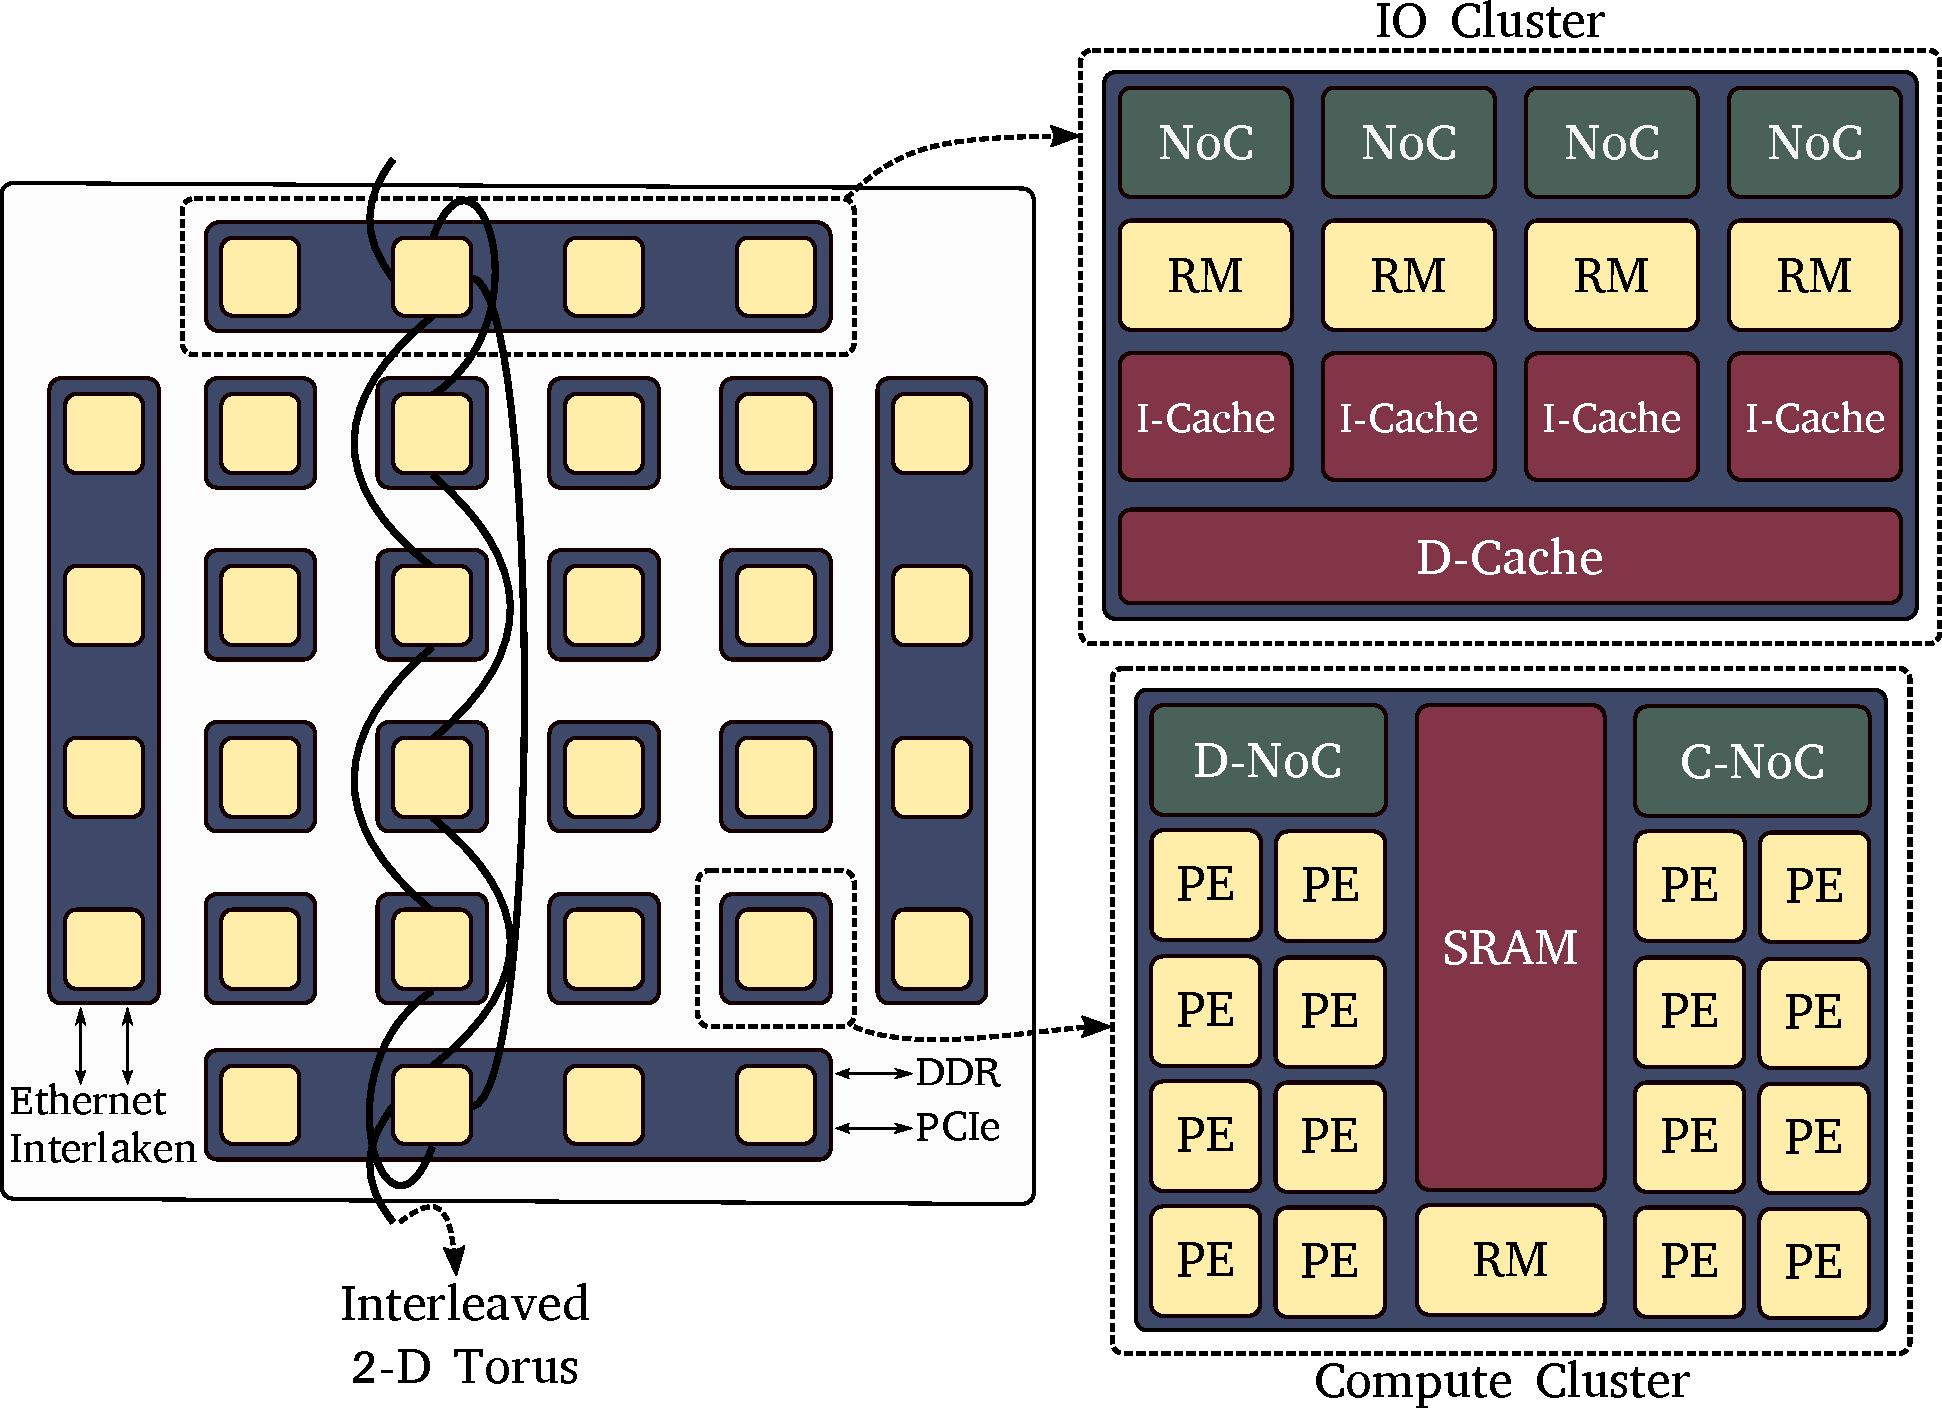
\includegraphics[width=.7\textwidth]{arch-mppa.pdf}%
		\fonte{\citeonline{Penna2018}.}%
	\end{figure}

	The \mppa is a high-performance, lightweight multicore processor
	developed by the French company Kalray.
	Developed to handle \mimd workloads, \mppa mixes features of
	multiprocessors and multicomputers on a single chip.
	Precisely, the multiprocessor model is used inside a cluster
	to coordinate the cores and the local resource balancing, and
	follows a multicomputer model in inter-cluster communication.

	\autoref{fig:mppa-arch} illustrates the version of \mppa architecture used, called Bostan.
	It has 256 general-purpose cores and 32 firmware cores, called \pes and \rms, respectively.
	The processor use 28~mm CMOS technology and all cores run at 500~MHz.
	Besides, all cores have caches and \mmus with software-managed \tlbs.
	Finally, the 288 cores are grouped into 16 \cclusters, dedicated to
	the payload, and 4 \ioclusters, responsible for communicating with peripherals.

	Each \ccluster features 16 \pes, an \rm, an \noc interface and 2~MB of \sram.
	The hardware does not support cache coherence to improve energy consumption.
	In contrast, \ioclusters have only 4 \rms with cache coherence support,
	4 \noc interfaces, and 4~MB of local \sram added to 4~GB of \dram.
	The address space on each cluster is private, forcing exchange messages
	by one of two different interleaved 2-D Torus \nocs.
	On the one hand, the \cnoc is exclusive to 64-bit control messages,
	usually used for synchronization.
	On the other hand, intense exchange data occurs through the \dnoc.
	Additionally, all clusters have available \dmas associated with each
	\noc interfaces to handle communication issues.

	As discussed in \autoref{sec.multicomputers-user-sw}, \noc interfaces
	expose communication resource to perform send and receive primitives
	like network interfaces.
	Accurately, they summarize the following resources:

	\begin{itemize}
		\item 128 slots for receiving commands;
		\item 256 slots for receiving data;
		\item 4 channels for sending commands;
		\item 8 channels for sending data, and;
		\item 8 $\mu$threads for sending asynchronous data (each of which must
			to be associated with a data transfer channel).
	\end{itemize}

	The configuration of these features is accomplished by a mix between
	writing on \dma registers and performing syscalls to a hypervisor
	that virtualizes the \mppa hardware.

\section{Nanvix: An Operating System for Lightweight Manycores}
\label{sec.nanvix}

	During the 1970s and 1980s, several \os initiatives began to emerge.
	To prevent \oss from being incompatible with each other, the \ieee creates
	the \posix standardization.
	\posix defines interfaces and behaviors expected from an \os, \eg creation
	and control of processes.
	Many of these systems ceased to exist, and new ones emerged, but \posix has
	consolidated and continues to extend to new concepts.

	The vast majority of current \oss are designed to work with a small number of cores.
	As the number of cores increases, certain parts of the \os require redesign.
	At some point, this rework will be unfeasible.
	This assertion led researchers to study design alternatives for the new era of
	processors~\cite{wentzlaff_factored_2009, baumann_multikernel:_2009, Wisniewski2014}.
	However, the focus of these \oss is on improving performance.
	Occasionally, aspects of hardware and design interfere with \os interfaces and behavior.
	Additionally, a lack of alternative \oss for \lightweight \manycores that balance the
	development cost requires from the user a considerable development and debugging effort.

	In this context, current research efforts on Nanvix \os focus on the
	programmability and portability	challenges that have arisen with
	\lightweight \manycores~\cite{christgau2017, gamell2012, serres2011}.
	We believe that significant barriers will still arise in this scenario, and
	the solution is to rethink \os design from scratch without losing back
	compatibility~\cite{penna:compas19, penna2019}.
	\autoref{fig:nanvix-goal} summaries the balancing of Nanvix \os goals.
	To achieve this balance, the Nanvix \os aims to improve programmability
	and software portability in lightweight manycores through a fully-featured
	\posix-compliant \os~\cite{penna:compas19}.

	\begin{figure}[!tb]
		\centering%
		\caption{Conceptual Goals of the Nanvix \os.}%
		\label{fig:nanvix-goal}%
		
\includegraphics[width=.55\textwidth]{nanvix-goal.pdf}%
		\fonte{VER COM O PEDRO COMO REFERENCIAR (REPOSITÓRIO NANVIX?).}%
	\end{figure}

	Three distinct layers of kernels make up the Nanvix \os.
	In a bottom-up approach of abstraction level, they are namely \textit{Nanvix \hal},
	\textit{Nanvix \microkernel}, and \textit{Nanvix \multikernel}.
	The next sections will introduce the concepts and problems addressed by
	each layer.

	\subsection{Nanvix Hardware Abstract Layer}
	\label{sec.hal}

		Nanvix \os proposes a generic and flexible \hal around the
		intrinsic architectural characteristics of the \lightweight \manycores.
		Currently, \hal has available all the essential modules to run standalone
		processes for the \mppa~\cite{DeDinechin2013-1}, \optimsoc~~\cite{Wallentowitz2013},
		and \hero~\cite{Kurth2017} platforms.
		Hence, in this undergraduate dissertation, we will focus on developing
		inter-cluster communication module for the \mppa processor.

		Unlike other approaches that aim to design a fully-featured \os~\cite{Baumann2009,kluge2014,nightingale2009,rhoden2011},
		the \hal belongs to one level below.
		It is the first layer on top of the hardware and should provide a standard
		view of these emerging processors for a client application, \eg \os.
		At this level, we do not protect internal structures with locks.
		Thus, the upper-level decides how to protect and multiplex \hal access.
		On the one hand, a traditional monolithic \os that implements a time-sharing
		behavior to access internal structures will need to apply locks manually.
		On the other hand, a master-slave \os not require such strict control,
		improving its performance.
		\autoref{fig:hal-overview} pictures the three logic layers of the \hal:

		\begin{figure}[!tb]
			\centering%
			\caption{Structural overview of the \hal.}%
			\label{fig:hal-overview}%
			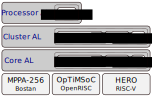
\includegraphics[width=.55\textwidth]{nanvix-hal-overview.pdf}%
			\fonte{VER COM O PEDRO COMO REFERENCIAR (REPOSITÓRIO NANVIX?).}%
		\end{figure}

		\begin{description}

			\item[Core Abstraction Layer]
				encapsulates the management of a single core.
				It provides a uniform view and maintenance routines for \tlbs, \mmu and cache,
				a rich support of handling exceptions/traps/interrupts, and
				access to \pmio.
				Therefore, some design decisions are made to create interfaces that are not
				dependent on the underlying hardware.
				For example, a context switch mechanism was not provided in the
				\textit{Core Package} because this would force the client \os
				to write code in assembly, hurting the conceptual idea of the \hal.

			\item[Cluster Abstraction Layer]
				encapsulates the management of characteristics that affect all cores in a cluster.
				It provides support for virtual memory, cross-core notification through events,
				clock counter fetching, and access to I/O resources such as \mmio and \dma.

			\item[Processor Abstraction Layer]
				embraces architectural features related to multiple clusters.
				The \textit{Inter-Cluster Communication Module}, the focus of
				this undergraduate dissertation, provide \noc identification routines and
				exports three main abstractions to allow synchronizaton and data
				exchange among clusters, based on ideas proposed along with the
				\nodeos distributed runtime system~\cite{DeDinechin2013-1}.

		\end{description}

	\subsection{Nanvix Microkernel}
	\label{sec.microkernel}

		The Nanvix \microkernel, running above the \hal, provide
		bare bones system abstractions to the client applications~\cite{penna:sbesc19}.
		Through a rich system call interface, it follows a Master-Slave \os model
		to avoid cache coherence issues present in manycores.
		The scope of the \microkernel is within a single cluster.
		System calls and internal subsystems manage local and shared resources
		available to all cores to maintain the coherence of the \os.
		\autoref{fig:microkernel-overview} pictures the five logic layers of the \microkernel:

		\begin{figure}[!tb]
			\centering%
			\caption{Concept Structural overview of the \microkernel.}%
			\label{fig:microkernel-overview}%
			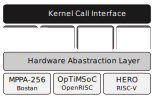
\includegraphics[width=.55\textwidth]{nanvix-microkernel-overview.pdf}%
			\fonte{VER COM O PEDRO COMO REFERENCIAR (REPOSITÓRIO NANVIX?).}%
		\end{figure}

		\begin{description}

			\item[IPC Facility]
				encapsulates the rest of this undergraduate dissertation, providing
				manipulation and protection of the inter-cluster communication abstractions.
				
			\item[Thread System]
				implements a rich mechanism to criation, management and protection of threads.
				This system features schedules, sleep, and wakeup routines of the user threads.
				
			\item[Memory System]
				provides a rich memory management and virtual memory support at cluster-level.
				It is based in a two-level paging scheme, supports pages of heterogeneous sizes
				and uses a capabilities system~\cite{Baumann2009} to keep track of permissions on pages.

			\item[Device System]
				controls the access to memory and port mapped devices, and provides
				mechanisms to forward the implementation of rich device drivers to user space.

			\item[Kernel Call Interface]
				isolates the \microkernel internal structures through a rich system call interface.
				This interface implements the Master-Slave \os model
				and decides whether or not a kernel call should be executed locally or remotely.

		\end{description}

		\autoref{fig:microkernel-execution} exemplifies a thread creation on Nanvix \microkernel.
		When a user thread makes a kernel call, a set of sanity checks are performed
		to ensure the integrity of the operation.
		After verifying the correctness of the parameters, the user thread notifies
		the kernel thread and waits locked.
		The kernel thread implements a producer/consumer policy and executes requests
		one at a time.
		When consuming a request, the master identifies it and performs the necessary operations.
		In the end, the kernel thread releases the requesting slave.
		Note that the master core always performs all operations that change internal
		\os structures.
		kernel calls that only query static parameters or structures (performing cache invalidation) are made locally.

		\begin{figure}[!tb]
			\centering%
			\caption{Execution example of the Nanvix \microkernel.}%
			\label{fig:microkernel-execution}%
			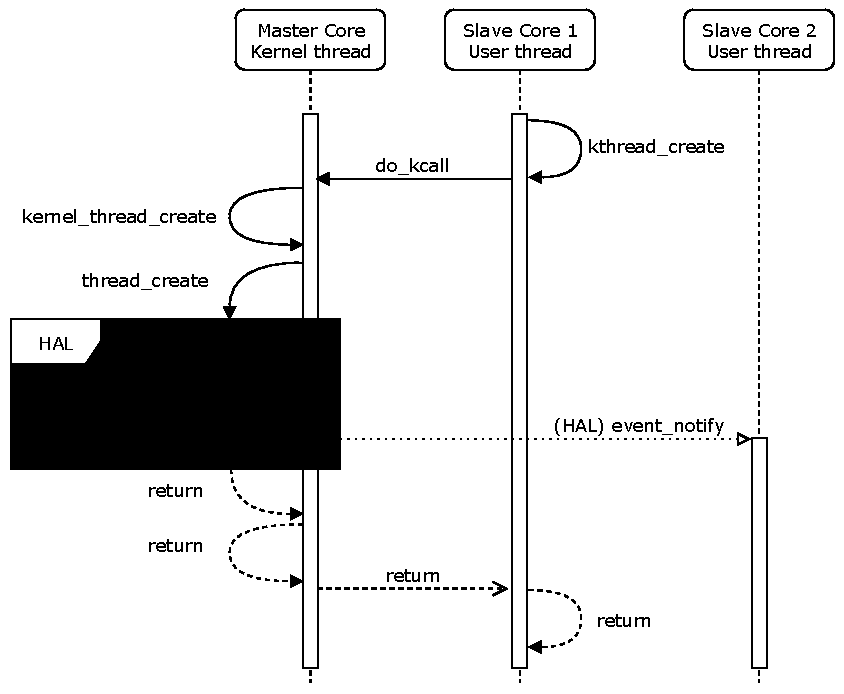
\includegraphics[width=.8\textwidth]{nanvix-microkernel-execution.pdf}%
			\fonte{Developed by the Author.}%
		\end{figure}

	\subsection{Nanvix Multikernel}
	\label{sec.multikernel}

		The Nanvix \multikernel follows a multikernel design, where \os services
		are scattered across clusters and interact with user processes through a
		Client-Server model.
		Ideally, \os services run in isolation from user processes.
		Via a message-passing approach, user processes request such services and
		cooperate with other processes.

		Research that explores the parallel and distributed nature of multicore and
		manycore processors inspires the Nanvix \multikernel~\cite{wentzlaff_factored_2009, baumann_multikernel:_2009, Wisniewski2014}.
		By treating the processor as a network of independent cores, it is possible
		to cover concepts of modern distributed systems.
		At this level of abstraction, the following distributed system concepts can be exploited:

		\begin{description}

			\item[Local Automation:] Each node can be independent of the other nodes, providing
				security, locking, access, integrity, and failover mechanisms.

			\item[Replication Independence:] Servers and data can be replicated across multiple
				nodes transparently and automatically synchronized.

			\item[Non-dependency on a central node:] When replicating servers, the system no
				longer relies on a central node.
				It eliminates the risk of having a single point of failure that would affect all other nodes.
				A central node could also become overloaded, resulting in loss of system performance.

			\item[Location Transparency:] Users should not need to know where the servers
				or data are located. For instance, a name server can control name resolution.

		\end{description}

		\autoref{fig:multikernel-overview} shows a possible configuration of a
		manycore using the Nanvix \multikernel.
		Clusters located at the corners of the processor run kernel services
		to better serve a nearby subset of clusters.
		In the other clusters, we can see the distribution of two distinct applications.
		An application does not necessarily need to use all cores in a cluster.
		Now, looking carefully at a cluster, we can see that Nanvix \microkernel
		always reserves a single core for kernel execution, making the other cores
		available for application execution.

		\begin{figure}[!tb]
			\centering%
			\caption{Possible configurations on Nanvix \multikernel.}%
			\label{fig:multikernel-overview}%
			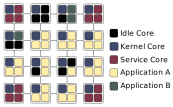
\includegraphics[width=.55\textwidth]{nanvix-multikernel-overview.pdf}%
			\fonte{VER COM O PEDRO COMO REFERENCIAR (REPOSITÓRIO NANVIX?).}%
		\end{figure}

		To enable Nanvix \os compliance with \posix, the Nanvix \multikernel is
		made up of high-level \os services that implement standardized interfaces.
		It exports both the client and server interfaces developed atop	the
		Nanvix \microkernel services.
		From this perspective, user applications are easily ported to run on
		Nanvix \multikernel, where client-side interfaces abstract the communication
		with servers distributed on the processor.
		\autoref{fig:multikernel-shm} exemplifies the existing layers to provide the \shm service.
		When opening an \shm, the client does not have to worry about where data
		will be allocated or whether other cores in other clusters are operating
		over the same memory region.
		Consequently, we provide greater programmability and software portability
		for manycores processors.

		\begin{figure}[!tb]
			\centering%
			\caption{\posix Compliance Example on Nanvix \multikernel.}%
			\label{fig:multikernel-shm}%
			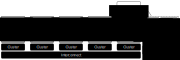
\includegraphics[width=.9\textwidth]{nanvix-multikernel-shm.pdf}%
			\fonte{VER COM O PEDRO COMO REFERENCIAR (REPOSITÓRIO NANVIX?).}%
		\end{figure}